\documentclass[10pt]{ctexart}
\usepackage{morelull}
\usepackage{enumerate}
\usepackage{bm}
\usepackage{makecell}
\usepackage{xcolor}
\usepackage{graphicx}
\usepackage{subfigure}
\usepackage{framed}%包中有添加文字背景色命令shaded
\colorlet{shadecolor}{MaterialBlue50}
\usepackage{tabularx}
\usepackage{multicol}  
\usepackage{multirow}
\usepackage{indentfirst}
\usepackage{amsmath,amssymb,amsthm,bm,bbding,pifont,dsfont}
\usepackage{mathtools}
\usepackage{tikz}
\newcommand{\abs}[1]{\left| #1 \right|}
\usepackage{caption}
\captionsetup[figure]{labelfont={bf},labelformat={default},labelsep=period,name={图}}
%定义选择题选项
\newcommand{\onech}[4]{
\renewcommand\arraystretch{1.4}
\begin{tabularx}{\linewidth}{XXXX}
\setlength\tabcolsep{0pt}
(A) #1 & (B) #2 & (C) #3 & (D) #4 \\
\end{tabularx}
\unskip \unskip}
\newcommand{\twoch}[4]{
\renewcommand\arraystretch{1.4}
\begin{tabularx}{\linewidth}{XX}
\setlength\tabcolsep{0pt}
(A) #1 & (B) #2 \\
(C) #3 & (D) #4
\end{tabularx}
\unskip \unskip}

\title{模型研究系列 \quad 角平分线四大模型}
\author{一粒沙整理\\安徽省霍邱县龙潭中心校}
\date{\today}



\begin{document}
\maketitle
\tableofcontents


\section{角平分线的相关重要知识点}
\begin{enumerate}
	\item 角平分线的定义
	\item 角平分线的性质定理
	\item 角平分线的判定定理
\end{enumerate}


\section{角平分线的相关模型}
\subsection[双垂模型]{角平分线上的点向两边作垂线( 双垂模型)}
【 {\heiti 模型基础}】

如图,$P$是$\angle MON$的平分线上一点,过点$P$作$PA\perp OM $于点$A$,$PB\perp BN $于点$B$.

结论:$PB=PA$.

\begin{flushright}
	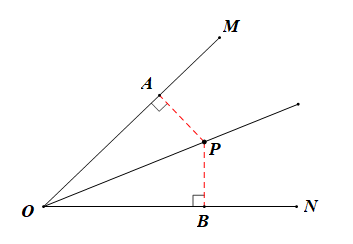
\includegraphics[scale=0.6]{figure/jiaopfxian01}
\end{flushright}

【 {\heiti 模型分析}】

利用角平分线的性质:角平分线上的点到角两边的距离相等,构造模型,为边相等、角相等、三角形全等创造更多的条件,进而可以快速找到解题的突破口。

【 {\heiti 模型实例}】
\begin{shaded}
	\begin{example}
	如图1,在$\triangle ABC$中,$\angle C=90^\circ$,$AD$平分$\angle CAB,BC=6,BD=4$,那么点$D$到直线$AB$的距离是$\underline{\hspace{1.5cm}}$;
	\end{example}
\end{shaded}

\begin{flushright}
	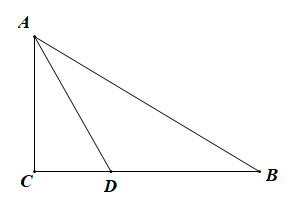
\includegraphics[scale=0.6]{figure/jiaopfxian02}
\end{flushright}

\begin{shaded}
	\begin{example}
	如图2,$\angle 1=\angle 2,\angle 3=\angle 4$. 求证:$AP$平分$\angle BAC$.
	\end{example}
\end{shaded}

\begin{flushright}
	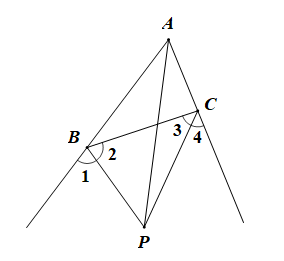
\includegraphics[scale=0.6]{figure/jiaopfxian03}
\end{flushright}


【 {\heiti 模型精炼}】
\begin{shaded}
	1.如图,在四边形$ABCD$中,$BC>AB$,$AD=DC$,$BD$平分$\angle ABC$。求证:$\angle BAD+\angle BCD=180^\circ$。
\end{shaded}

\begin{flushright}
	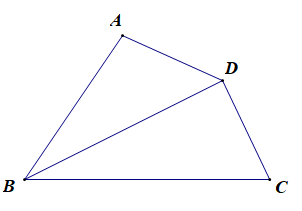
\includegraphics[scale=0.6]{figure/jiaopfxian04}
\end{flushright}

\begin{shaded}
   2.如图,$\triangle ABC$的外角$\angle ACD$的平分线$CP$与内角$\angle ABC$的平分线$BP$交于点$P$,若$\angle BPC=40^\circ$,则$\angle CAP=$$\underline{\hspace{1.5cm}}$.
\end{shaded}

\begin{flushright}
	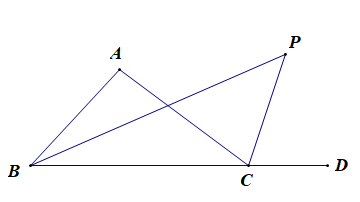
\includegraphics[scale=0.6]{figure/jiaopfxian05}
\end{flushright}

\begin{shaded}
  3.如图,正方形$ABCD$的边长为4,$\angle DAC$的平分线交$DC$于点$E$,若点$P,Q$分别是$AD$和$AE$上的动点,则$PQ+PD$的最小值是$\underline{\hspace{1.5cm}}$.
\end{shaded}

\begin{flushright}
	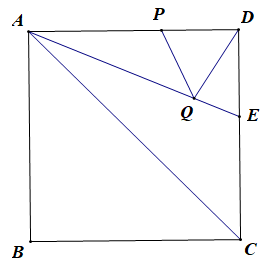
\includegraphics[scale=0.6]{figure/jiaopfxian06}
\end{flushright}

\subsection[单垂模型]{角平分线+垂线构造等腰三角形( 单垂模型)}

【 {\heiti 模型基础}】

如图,$P$是$MON$的平分线上一点,$AP\perp OP$于$P$点,延长$AP$于点$B$.

结论:$\triangle AOB$是等腰三角形.

\begin{flushright}
	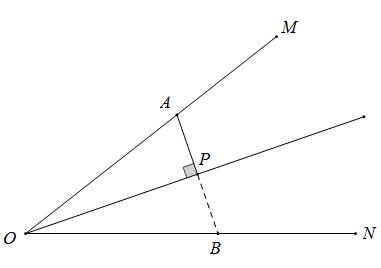
\includegraphics[scale=0.6]{figure/jiaopfxian07}
\end{flushright}

【 {\heiti 模型分析}】

构造此模型可以利用等腰三角形的“三线合一”,也可以得到两个全等的直角三角形,进而得到对应边、对应角相等。这个模型巧妙地把角平分线和三线合一联系了起来。

【 {\heiti 模型实例}】

如图,已知等腰直角三角形$ABC$中,$\angle A=90^\circ$,$AB=AC$,$BD$平分$\angle ABC$,
$CE\perp BD$,垂足为$E$.

求证:$BD=2CE$.

\begin{flushright}
	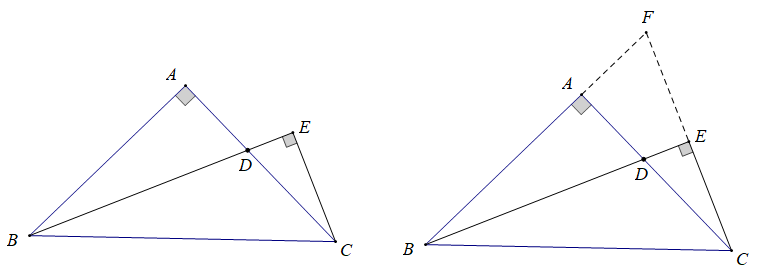
\includegraphics[scale=0.6]{figure/jiaopfxian08}
\end{flushright}

【 {\heiti 模型精炼}】
\begin{shaded}
1.如图,在$\triangle ABC$中,$BE$是角平分线,$AD\perp BE$,垂足为$D$。

求证:$\angle 2=\angle 1+\angle C $.
\end{shaded}

\begin{flushright}
	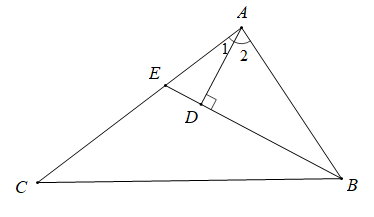
\includegraphics[scale=0.6]{figure/jiaopfxian09}
\end{flushright}

\begin{shaded}
2.如图,在$\triangle ABC$中,$\angle ABC=3\angle C$,$AD$是$\angle BAC$的平分线,$BE\perp AD$于点$E$。
 
求证:$BE=\dfrac{1}{2}(AC-AB)$.
\end{shaded}

\begin{flushright}
	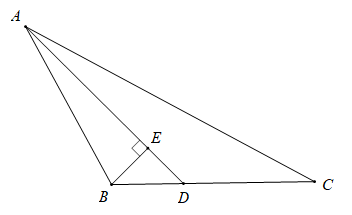
\includegraphics[scale=0.6]{figure/jiaopfxian10}
\end{flushright}

\subsection[双等模型]{截长补短构造对称全等( 双等模型)}

【 {\heiti 模型基础}】

如图,$P$是$\angle MON$的平分线上一点,点$A$是射线$OM$上任意一点,在$ON$
上截取$OB=OA$,连接$PB$.

结论:$\triangle OPB\cong \triangle OPA$.

\begin{flushright}
	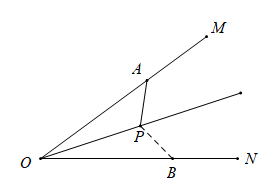
\includegraphics[scale=0.6]{figure/jiaopfxian11}
\end{flushright}

【 {\heiti 模型分析}】

利用角平分线图形的对称性,在角的两边构造对称全等三角形,可以得到对应边、对应角相等。利用对称性把一些线段或角进行转移,这是经常使用的一种解题技巧。

【 {\heiti 模型实例}】
\begin{shaded}
(1)图1所示,在$\triangle ABC$中,$AD$是$\triangle ABC$的外角平分线,$P$是$AD$上异于点$A$的任意一点,试比较$PB+PC$与$AB+AC$的大小,并说明理由;

(2)如图2所示, $AD$是$\triangle ABC$的内角平分线,其他条件不变,试比较$PC-PB$与$AC-AB$的大小,并说明理由。
\end{shaded}

\begin{center}
	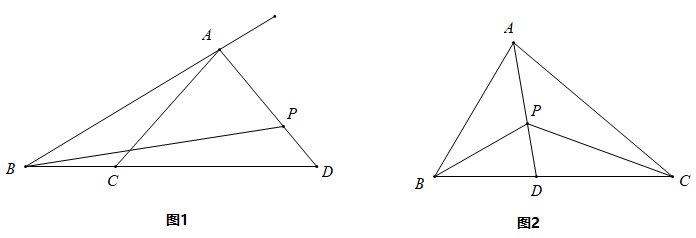
\includegraphics[scale=0.6]{figure/jiaopfxian12}
\end{center}

【 {\heiti 模型精炼}】

\begin{shaded}
1.已知,在$\triangle ABC$中,$\angle A=2\angle B$,$CD$是$\angle ACB$的平分线,$AC=16$,$AD=8$. 求线段$BC$的长。
\end{shaded}

\begin{flushright}
	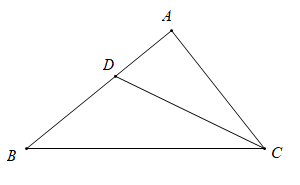
\includegraphics[scale=0.6]{figure/jiaopfxian13}
\end{flushright}

\begin{shaded}
2.已知,在$\triangle ABC$中,$AB=AC$,$\triangle A=108^\circ$,$BD$平分$\angle ABC$. 求证:$BC=AB+CD$.
\end{shaded}

\begin{flushright}
	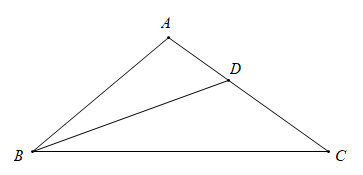
\includegraphics[scale=0.6]{figure/jiaopfxian14}
\end{flushright}

\begin{shaded}
3.如图所示,在$\triangle ABC$中,$\angle A=100^\circ$,$\angle A=40^\circ$,$BD$是$\angle ABC$的平分线,延长$BD$至$E$,$DE=AD$.求证:$BC=AB+CE$.
\end{shaded}

\begin{flushright}
	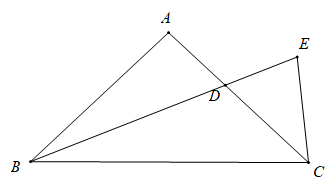
\includegraphics[scale=0.6]{figure/jiaopfxian15}
\end{flushright}

\begin{shaded}
4.如图,梯形$ABCD$中,$AD//BC$,点$E$在$CD$上,且$AE$平分$\angle BAD$,$BE$平分$\angle ABC$,求证:$AD=AB-BC$.
\end{shaded}

\begin{flushright}
	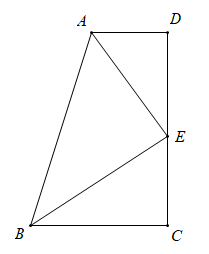
\includegraphics[scale=0.6]{figure/jiaopfxian16}
\end{flushright}




\subsection[双平模型]{角平分线+平行线( 双平模型)}

【 {\heiti 模型基础}】

如图,$P$是$\angle MON$的平分线上一点,过点$P$作$PQ//ON$,交$OM$于点$Q$.

结论:$\triangle POQ$是等腰三角形.

\begin{flushright}
	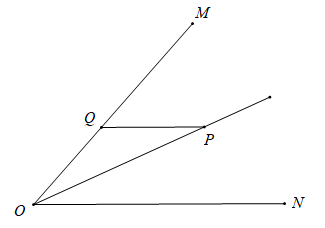
\includegraphics[scale=0.6]{figure/jiaopfxian17}
\end{flushright}

【 {\heiti 模型分析}】

有角平分线时,常过角平分线上一点作角的一边的平行线,构造等腰三角形,为证明结论提供更多的条件,体现了角平分线与等腰三角形之间的密切关系。


【 {\heiti 模型实例}】

\begin{shaded}
解答下列问题:

(1)如图1所示,在$\triangle ABC$中,$EF//BC$,点$D$在$EF$上,$BD,CD$分别平分$\angle ABC,\angle ACB$,写出线段$EF$与$BE,CF$有什么数量关系;

(2)如图2所示,$BD$平分$\angle ABC$,$CD$平分$\angle ACG$,$DE//BC$交$AB$于点$E$,交$AC$于点$F$,线段$EF$与$BE,CF$有什么数量关系?并说明理由;

(3)如图3所示,$BD,CD$分别为外角$\angle CBM,\angle BCN$的平分线,$DE//BC$交$AB$延长线于点$E$,交$AC$延长线于点$F$,直接写出线段$EF$与$BE,CF$有什么数量关系? 
\end{shaded}

\begin{flushright}
	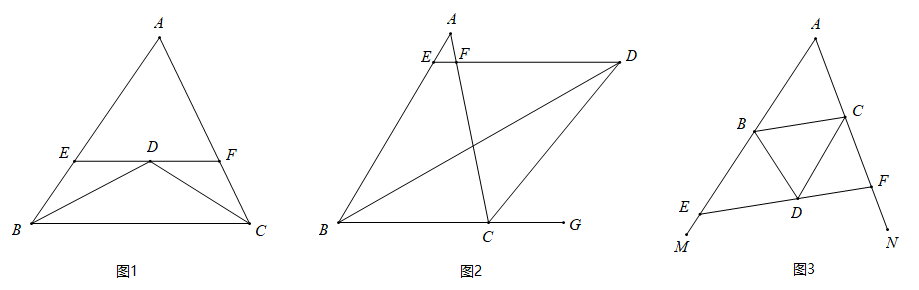
\includegraphics[scale=0.6]{figure/jiaopfxian18}
\end{flushright}

【 {\heiti 模型精炼}】

\begin{shaded}
1.如图,在$\triangle ABC$中,$∠\angle ABC,\angle ACB$ 的平分线交于点$E$,过点$E$作$EF//BC$,交$AB$于点$M$,交$AC$于点$N$.若$BM+CN=9$,则线段$MN$的长为$\underline{\hspace{1.5cm}}$.
\end{shaded}

\begin{flushright}
	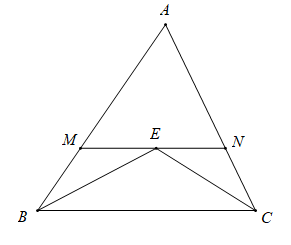
\includegraphics[scale=0.6]{figure/jiaopfxian19}
\end{flushright}

\begin{shaded}
2.如图,在$\triangle ABC$中,$AD$平分$\angle BAC$,点$E,F$分别在$BD,AD$上,$EF//AB$,且$DE=CD$.

求证:$EF=AC$.
\end{shaded}

\begin{flushright}
	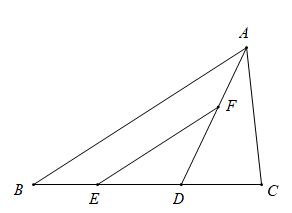
\includegraphics[scale=0.6]{figure/jiaopfxian20}
\end{flushright}

\begin{shaded}
3.如图,梯形$ABCD$中,$AD//BC$,点$E$在$CD$上,且$AE$平分$\angle BAD$,$BE$平分$\angle ABC$.

求证:$AD=AB-BC$.
\end{shaded}

\begin{flushright}
	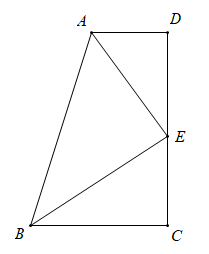
\includegraphics[scale=0.6]{figure/jiaopfxian16}
\end{flushright}

\begin{shaded}
4.如图,在矩形$ABCD$中,$\angle BAD$的平分线交$BC$于点$E$,交$DC$的延长线于点$F$,点$G$是$EF$的中点,求$\angle BDG$的度数。
\end{shaded}

\begin{flushright}
	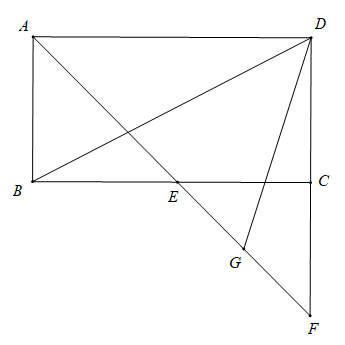
\includegraphics[scale=0.6]{figure/jiaopfxian21}
\end{flushright}

\end{document}